%------------------------------------------------------------------------------
\section{Software Engineering for Economists}
%------------------------------------------------------------------------------
I teach students basic software engineering skills to tackle computer-intensive economic research projects. During lectures and a group project, we explore the following set of topics:
%
\begin{multicols}{2}
\begin{itemize}
\item Version Control
\item Unit Testing
\item Debugging and Profiling
\item Code Documentation
\item Design Patterns
\item Data Management
\item Cloud Computing
\item High Performance Computing
\end{itemize}
\end{multicols}
%
\noindent These basic techniques allow us to leverage tools from computational science, increase the transparency of our implementations, and ensure the recomputability of results. Thus, they expand the set of possible economic questions that we can address and improve the quality of our answers.\\

\noindent This class requires a basic knowledge of the \textit{Ubuntu} operating system and \textit{Python} programming language. For novices, we offer a \textit{Software Engineering Bootcamp} in the week before regular classes start to catch up on these basics.\\\newline
%
\noindent Updated information and additional background material is provided on the course website:
\begin{center}
\url{https://github.com/softEcon}
\end{center}\vspace{0.3cm}
%------------------------------------------------------------------------------
\subsection{Course}
%------------------------------------------------------------------------------

\begin{boenumerate}
\item \textit{How would you rate the course overall?}
%------------------------------------------------------------------------------
%------------------------------------------------------------------------------
\begin{figure}[h!]\centering
\scalebox{0.5}{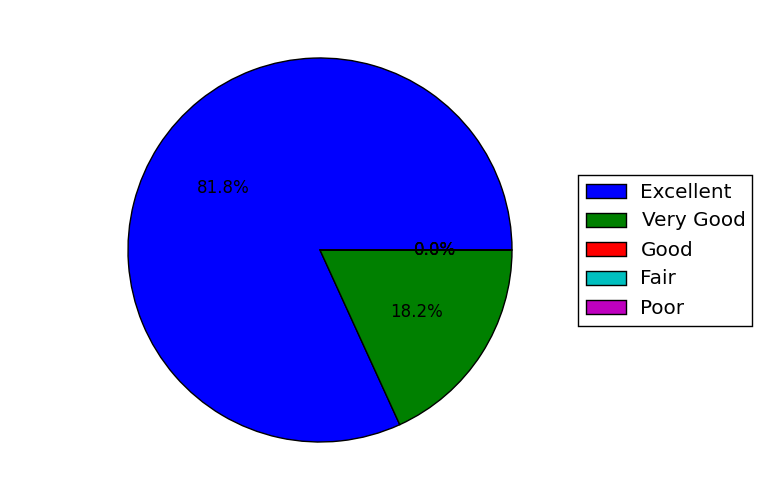
\includegraphics{../graphs/overall.png}}\hspace{0.75cm}
\begin{center}
\begin{minipage}[t]{0.85\columnwidth}\vspace{-0.75cm}
\item\scriptsize{\textbf{Notes:} Based on 11 student responses. }
\end{minipage}
\end{center}
\end{figure}
%------------------------------------------------------------------------------
%------------------------------------------------------------------------------
\item \textit{Which part of the University are you from?}

\begin{figure}[h!]\centering
\scalebox{0.5}{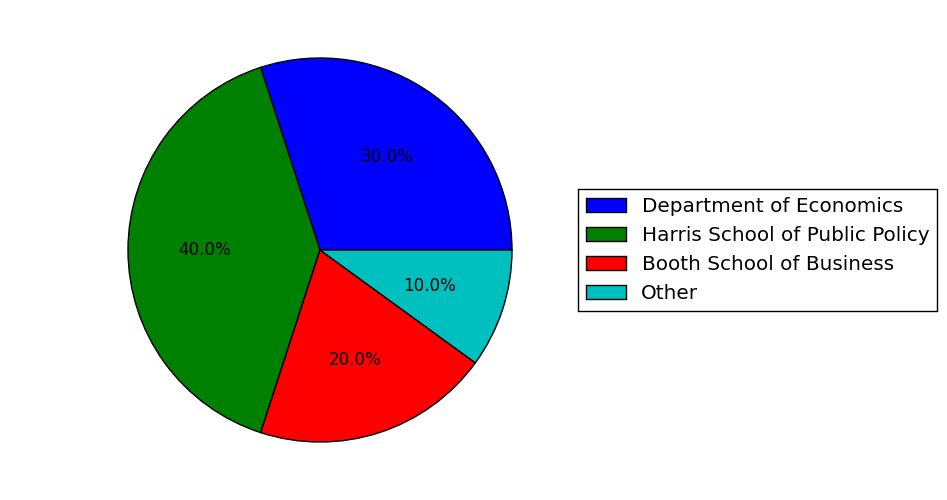
\includegraphics{../graphs/part_univ.png}}\hspace{0.75cm}
\begin{center}
\begin{minipage}[t]{0.85\columnwidth}\vspace{-0.75cm}
\item\scriptsize{\textbf{Notes:} Based on 10 student responses, possible choices were: \emph{Excellent, Very Good, Good, Fair, Poor}}
\end{minipage}
\end{center}
\end{figure}
\newpage
%------------------------------------------------------------------------------
%------------------------------------------------------------------------------
\item \textit{Relative to your other classes, how useful was this course?}

\begin{figure}[h!]\centering
\scalebox{0.5}{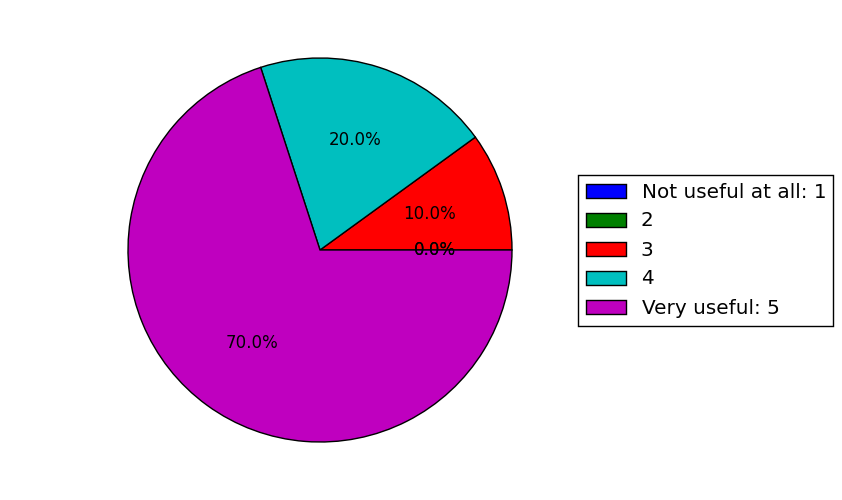
\includegraphics{../graphs/useful.png}}\hspace{0.75cm}
\begin{center}
\begin{minipage}[t]{0.85\columnwidth}\vspace{-0.75cm}
\item\scriptsize{\textbf{Notes:} Based on 10 student responses, possible choices were: \emph{Not useful at all: 1, 2, 3, 4, Very useful: 5}}
\end{minipage}
\end{center}
\end{figure}

%------------------------------------------------------------------------------
%------------------------------------------------------------------------------
\item \textit{How well did Philipp meet his goal ...}
\begin{itemize}
\item \textit{to be well organized?}

\begin{figure}[h!]\centering
\scalebox{0.5}{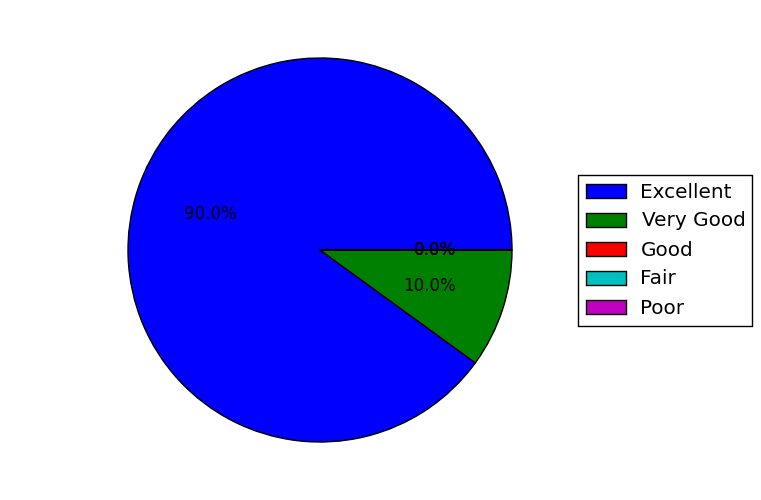
\includegraphics{../graphs/organized.png}}\hspace{0.75cm}
\begin{center}
\begin{minipage}[t]{0.85\columnwidth}\vspace{-0.75cm}
\item\scriptsize{\textbf{Notes:} Based on 10 student responses, possible choices were: \emph{Excellent, Very Good, Good, Fair, Poor} }
\end{minipage}
\end{center}
\end{figure}

%------------------------------------------------------------------------------
%------------------------------------------------------------------------------
\item \textit{to present the material at the right speed?}

\begin{figure}[h!]\centering
\scalebox{0.5}{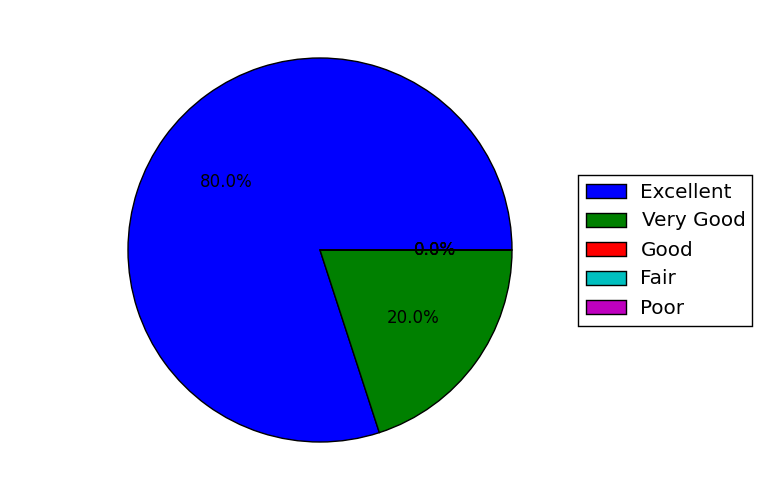
\includegraphics{../graphs/speed.png}}\hspace{0.75cm}
\begin{center}
\begin{minipage}[t]{0.85\columnwidth}\vspace{-0.75cm}
\item\scriptsize{\textbf{Notes:} Based on 10 student responses, possible choices were: \emph{Excellent, Very Good, Good, Fair, Poor} }
\end{minipage}
\end{center}
\end{figure}

%------------------------------------------------------------------------------
%------------------------------------------------------------------------------
\item \textit{to present the material clearly and understandable?}

\begin{figure}[h!]\centering
\scalebox{0.5}{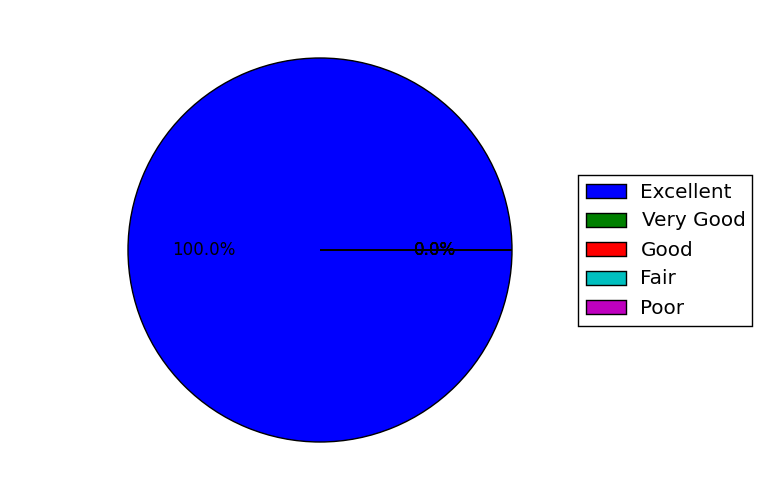
\includegraphics{../graphs/clearly.png}}\hspace{0.75cm}
\begin{center}
\begin{minipage}[t]{0.85\columnwidth}\vspace{-0.75cm}
\item\scriptsize{\textbf{Notes:} Based on 10 student responses, possible choices were: \emph{Excellent, Very Good, Good, Fair, Poor} }
\end{minipage}
\end{center}
\end{figure}
%------------------------------------------------------------------------------
%------------------------------------------------------------------------------
\item \textit{to be accessible outside of class?}

\begin{figure}[h!]\centering
\scalebox{0.5}{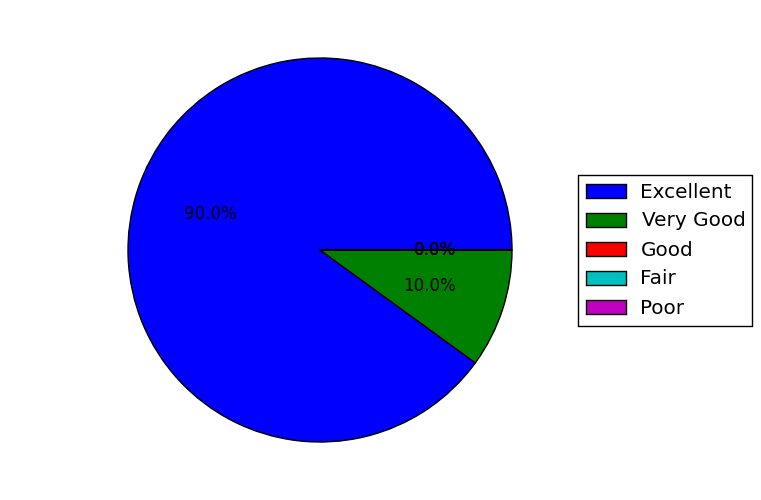
\includegraphics{../graphs/access.png}}\hspace{0.75cm}
\begin{center}
\begin{minipage}[t]{0.85\columnwidth}\vspace{-0.75cm}
\item\scriptsize{\textbf{Notes:} Based on 10 student responses, possible choices were: \emph{Excellent, Very Good, Good, Fair, Poor} }
\end{minipage}
\end{center}
\end{figure}







\end{itemize}
%------------------------------------------------------------------------------
%------------------------------------------------------------------------------
\item \textit{How has the course helped with your PhD research?}
\begin{itemize}
\item Improve my code, make it scalable and transparent. Better understanding of the different optimization routines. Better productivity.
\item I think the course is very helpful overall. It helps to get familiar with how to use \textit{Python} to implement economic models. Besides, I also learned a lot about how to organize my project well. This will help me to save a lot of time.
\item Exposure to useful technical tools.
\item I had been thinking of doing some projects that require generalized Roy models. Seeing how to implement these models in a proficient way has definitely helped me in two ways. First, the likelihood that I will do so has increased, and in terms of my own productivity while doing and computation intensive project since I learned quite a few useful tricks form Philipp.
\item Introduced tools and habits that will save an enormous amount of time from having to spent on routines/practical/logistical tasks, time which can instead be spent on work more directly meaningful of high quality research.
\item The course was extremely helpful in furthering computational abilities needed for exploring my project, and providing a clear implementation of a well known model computationally.
\item I learned how to use a very good and free software that is \textit{Python}. It contains lots of packages I'm interested in such as network analysis. I also learned how to use \textit{GitHub} to share data with my coauthors and save previous versions as backup.
\item It helps us understand some basic software engineering skills. Make me more interested in doing some computation-intensive economic research in the future.
\item It was essential for coding.
\item Taught me skills and tools to improve the quality of empirical work.
\end{itemize}
%------------------------------------------------------------------------------
%------------------------------------------------------------------------------
\item \textit{Do you have any additional recommendations for Philipp?}
\begin{itemize}
\item No. He is amazing and very helpful and always available.
\end{itemize}
%------------------------------------------------------------------------------
%------------------------------------------------------------------------------
\item \textit{What aspects of the course should be changed?}
\begin{itemize}
\item The source was changed all the time. First, the website, then \textit{GitHub}. That was suboptimal. Also, more programming principles would be nice, and maybe less cloud computing.
\item Everything looks good. I might continue to audit the next year's class.
\item Should be taught in the autumn to provide maximum benefit to second year students (lean the skills before they start their research). Perhaps introduce (optional) homework where a problem is posted and then students can submit their solutions for how they would tackle the problem. Then discuss in class the various pros and cons of the different methods.
\item None. This was really a great course.
\item I do believe that \textit{Git} setup should be at the beginning and very carefully set up.
\item Maybe more \textit{GUI}. \textit{Vagrant} made my computer slow but I understand how useful it was. Maybe each student should work on their own project.
\end{itemize}
%------------------------------------------------------------------------------
%------------------------------------------------------------------------------
\item \textit{What aspects of the course should be retained?}
\begin{itemize}
\item The wide range of topics covered.
\item All.
\item Using real examples like the \textit{grmToolbox} is really good!
\end{itemize}
\end{boenumerate}

